\documentclass{article}

% if you need to pass options to natbib, use, e.g.:
%     \PassOptionsToPackage{numbers, compress}{natbib}
% before loading neurips_2026

% The authors should use one of these tracks.
% Before accepting by the NeurIPS conference, select one of the options below.
% 0. "default" for submission
\usepackage{neurips_2026}
% the "default" option is equal to the "main" option, which is used for the Main Track with double-blind reviewing.

\usepackage[utf8]{inputenc} % allow utf-8 input
\usepackage[T1]{fontenc}    % use 8-bit T1 fonts
\usepackage{hyperref}       % hyperlinks
\usepackage{url}            % simple URL typesetting
\usepackage{booktabs}       % professional-quality tables
\usepackage{multirow}       % multi-row table cells
\usepackage{amsmath}        % math environments and \text
\usepackage{amsfonts}       % blackboard math symbols
\usepackage{nicefrac}       % compact symbols for 1/2, etc.
\usepackage{microtype}      % microtypography
\usepackage{xcolor}         % colors
\usepackage{algorithm}      % algorithm environment
\usepackage{algorithmic}    % algorithmic pseudocode
\usepackage{graphicx}       % graphics

\title{SharQ：连接激活稀疏性与 FP4 量化的 LLM 推理方法}

\author{%
  Anonymous Authors \\
  Anonymous Institution \\
  \texttt{anonymous@example.com} \\
}

\begin{document}

\maketitle

\begin{abstract}
\end{abstract}

\section{引言}

大语言模型推理的主要开销来自线性层。随着模型规模和在线服务需求持续增长，降低矩阵乘法成本已经成为推理系统中的核心问题。低比特浮点格式和半结构化稀疏是两个越来越实际的方向，因为它们不再只是算法层面的压缩技术，也逐渐成为硬件直接支持的执行路径。NVFP4、MXFP4 和 HiF4 等块缩放 FP4 格式在提高计算密度的同时保留了一定的浮点动态范围，而 N:M 半结构化稀疏则可以利用现代 Tensor Cores 上的稀疏矩阵乘法能力。这些趋势共同指向一个很自然的目标：在 LLM 推理中结合 FP4 量化与硬件支持的稀疏计算。

然而，将 FP4 量化直接应用到激活上仍然困难。相比权重，激活依赖于当前输入，并且经常包含少量大幅值 outliers。由于块缩放 FP4 通常由局部块中的最大值决定缩放因子，这些 outliers 会主导整个块的 scale，从而降低普通激活值可用的有效精度。已有 LLM 量化工作，包括 LLM.int8()、SmoothQuant、AWQ、GPTQ、OmniQuant、QuaRot 和 SpinQuant，从不同角度说明了 outliers 和激活分布是低比特推理中的关键障碍。混合精度或 outlier-aware 路径可以缓解这类误差，但往往会引入额外存储、不规则访存或辅助 kernel，这些代价并不适合一个高效的 FP4 执行流水线。

激活稀疏提供了一个看似自然的替代思路。在许多 LLM 层中，最大幅值的激活值本身是稀疏的，并且对输出贡献较大。这意味着我们似乎可以将这些大值路由到稀疏路径，并利用 N:M sparse Tensor Core 指令加速计算。但在 training-free 场景下，直接激活稀疏化通常过于有损。与 SparseGPT、Wanda 等权重稀疏方法不同，激活 mask 无法离线固定或通过校准优化，而必须根据当前输入在线生成。同时，DejaVu、PowerInfer 等推理阶段激活稀疏方法更多依赖粗粒度预测或路由，而细粒度 N:M 激活 mask 还需要满足严格的硬件模式，并且必须在推理关键路径上以很低开销生成。如果稀疏路径只是保留最大值并丢弃其余激活，大量中等幅值信息会被直接丢失，从而造成明显精度下降。

因此，问题并不只是如何把稀疏和量化简单组合起来，而是如何定义二者在同一个近似问题中的角色。在 sparse FP4 路径中，稀疏化会先改变激活的局部分布，随后 FP4 量化又会基于这个改变后的分布选择 scale。最终误差并不是独立的稀疏误差和独立的量化误差之和，而是二者相互耦合后的结果。一个有效设计需要在保留 sparse FP4 硬件收益的同时，保存无法被稀疏表示完整表达的激活信息。

本文提出 SharQ，一种 training-free 的 LLM 推理方法，通过在线 sparse--dense 分解连接激活稀疏性与 FP4 量化。SharQ 的重点不在于提出抽象意义上的激活分解，而在于让这种分解同时具备输入自适应性、硬件合法性和量化感知能力。对于每个激活，SharQ 在线生成满足 N:M 约束的 mask，提取由 outliers 主导的 sparse backbone。该 backbone 随后被量化并通过 sparse FP4 GEMM 执行。与直接对未量化稀疏值做残差不同，SharQ 将 dense residual 定义在量化后的 sparse backbone 之上。因此，该 residual 同时包含 sparse mask 之外的激活信息，以及 sparse FP4 路径本身引入的量化误差。最后，dense FP4 GEMM 将 residual contribution 累加到 sparse output 上。

这一设计带来两个实际优势。首先，稀疏 mask 由当前激活在线决定，因此 SharQ 不需要校准数据、微调或离线学习的固定 mask。这也解释了为什么同一机制可以泛化到 dense decoder-only 模型、Mixture-of-Experts 模型、Wan2.2 等文生视频模型以及不同 FP4 数值格式。其次，SharQ 的实现围绕真实 kernel 约束设计：mask 选择、稀疏输入压缩和 residual 准备被融合到同一准备阶段；两个路径共享 FP4 weight payload，并使用路径特定的 scale view；dense residual 路径直接累加到 sparse output 中。因此，SharQ 不只是一个激活近似策略，也是一个面向硬件执行的推理原语。

本文的主要贡献如下：
\begin{itemize}
  \item 提出 SharQ，一种 training-free 的 FP4 推理方法，将激活在线分解为 N:M sparse backbone 和 dense FP4 residual。
  \item 将 residual 定义在量化后的 sparse backbone 之上，使 dense path 能够同时补偿 mask 引起的激活信息损失和 sparse-path FP4 量化误差。
  \item 设计了高效实现，包括融合的激活准备、带路径特定 scale 的共享 FP4 权重，以及基于累加的 residual compensation，并在多种模型架构、FP4 格式和推理设置下进行验证。
\end{itemize}

\section{相关工作}

\subsection{量化}

\subsection{稀疏性}

\subsection{细粒度数值格式与硬件支持}

\section{方法}

\subsection{预备知识}

考虑 Transformer 模型中的一个线性层。给定输入激活矩阵
$\mathbf{X} \in \mathbb{R}^{T \times K}$ 和权重矩阵
$\mathbf{W} \in \mathbb{R}^{K \times D}$，其全精度输出为
\begin{equation}
  \mathbf{Y} = \mathbf{X}\mathbf{W}.
  \label{eq:linear-layer}
\end{equation}
本文研究如何在不重新训练模型的情况下，利用低比特量化和硬件支持的半结构化稀疏来近似这一计算。记
$\mathcal{H}$ 为目标数值格式、稀疏模式和矩阵乘 kernel 共同决定的可实现计算集合，则优化目标可以写为
\begin{equation}
  \min_{\widehat{\mathbf{Y}} \in \mathcal{H}}
  \| \mathbf{Y} - \widehat{\mathbf{Y}} \|_F^2 ,
  \label{eq:hardware-objective}
\end{equation}
其中 $\widehat{\mathbf{Y}}$ 由量化后的激活、量化后的权重以及满足硬件约束的稀疏模式共同产生。

我们首先回顾 group-wise 对称量化。对于一个局部组 $\mathcal{G}$ 和一个低比特码本
$\mathcal{B}$，缩放因子通常由该组内的最大幅值决定。对组内元素 $x_i$，该过程可以表示为
\begin{equation}
  s_{\mathcal{G}} =
  \frac{\max_{i \in \mathcal{G}} |x_i|}{\alpha_{\mathcal{B}}},
  \quad
  q_i =
  \Pi_{\mathcal{B}}\left(\frac{x_i}{s_{\mathcal{G}}}\right),
  \quad
  \widehat{x}_i = s_{\mathcal{G}} q_i ,
  \label{eq:group-quant}
\end{equation}
其中 $\alpha_{\mathcal{B}}$ 表示码本中可表示的最大幅值，
$\Pi_{\mathcal{B}}(\cdot)$ 表示投影到最近的可表示值。NVFP4 和 HiF4 等 block-scaled FP4
格式在这一思想上进一步细化：它们为小块张量分配细粒度缩放因子，同时保持适合 Tensor Core 的低比特操作数。例如，NVFP4
将 FP4 数值与局部块缩放因子以及二级全局缩放因子结合，从而相比单一缩放因子的 FP4 表示获得更好的动态范围。具体编码细节将在附录中说明。

N:M 半结构化稀疏是另一类面向硬件的 primitive。它要求每个连续的 $M$ 个元素，或硬件定义的基本单元，只保留
$N$ 个非零值。由此得到的稀疏矩阵乘可以通过专门的 Tensor Core 指令加速。传统稀疏推理方法通常离线学习或校准一个固定
mask，并在所有输入上复用该 mask。与之不同，本文关注 activation sparsity，即根据当前输入激活的数值在线生成 mask。若
$\mathbf{M}(\mathbf{X})$ 是满足目标 N:M 约束的动态 mask，则稀疏激活路径可以写为
\begin{equation}
  \mathbf{X}_{\mathrm{sp}} =
  \mathbf{M}(\mathbf{X}) \odot \mathbf{X},
  \quad
  \mathbf{M}(\mathbf{X}) \in \mathcal{S}_{N:M},
  \label{eq:dynamic-mask}
\end{equation}
其中 $\odot$ 表示逐元素乘法，$\mathcal{S}_{N:M}$ 表示所有合法的半结构化 mask 集合。

在实际系统中，量化和稀疏并不是两个彼此独立的近似。新一代硬件允许低比特格式与半结构化稀疏组合使用，例如 NVFP4
与 4:8 in pairs 稀疏模式，以及 HiF4 与标准 2:4 稀疏模式。直接的稀疏量化激活路径可以概括为
\begin{equation}
  \widehat{\mathbf{Y}}_{\mathrm{sq}} =
  \mathrm{GEMM}\left(
    \mathcal{Q}_x(\mathbf{M}(\mathbf{X}) \odot \mathbf{X}),
    \mathcal{Q}_w(\mathbf{W})
  \right).
  \label{eq:direct-sparse-quant}
\end{equation}
然而，一旦激活被稀疏化，其局部数值分布和缩放因子选择也会随之改变。因此，最终误差并不能简单看作独立稀疏误差与独立量化误差之和。这种误差耦合正是后续章节引入 decomposition 设计的动机。

\subsection{动机}

上述形式化表明，低比特量化和半结构化稀疏为线性层推理提供了明确的硬件加速路径。然而，直接将激活压缩为单一的低比特或稀疏表示通常难以同时满足精度和效率需求。其根本原因在于，大模型激活同时具有少数大幅值
outliers 和大量中小幅值元素：前者主导局部动态范围，并构成可被稀疏提取的重要信号；后者虽然单个幅值较小，却共同承载了不可忽略的输出信息。因此，如何在硬件友好的约束下同时处理这两类信号，是本文方法设计的出发点。

\textbf{激活离群值会削弱 FP4 量化的有效分辨率。}
在 group-wise FP4 量化中，缩放因子通常由组内最大幅值决定。因此，少数
outliers 会迫使整个 group 使用较大的 scale，使得普通幅值元素被映射到更粗糙的量化间隔中，产生明显的量化误差。一类自然的补救方式是对
outliers 引入更高精度表示或额外计算路径，但这往往会带来混合精度存储、额外
kernel 或不规则数据访问，从而削弱统一 FP4 Tensor Core 路径的硬件效率。换言之，关键挑战并不只是识别
outliers，而是在硬件友好的低比特执行路径中有效处理它们。

\textbf{动态激活稀疏性很难直接转化为 training-free 的 N:M 稀疏。}
本文所利用的激活稀疏性并不是大量精确零值，而是少数大幅值
outliers 的稀疏分布。由于这些 outliers 通常主导输出贡献，可以通过
top-$k$ 或满足 N:M 约束的局部选择规则从当前激活中在线提取，形成输入自适应的
sparse mask。然而，在线 mask 生成位于推理关键路径上，必须保持极低开销，难以依赖复杂搜索或迭代优化。已有
activation sparsity 方法因此更多采用结构化或粗粒度形式，而细粒度 N:M mask 的优化主要出现在权重稀疏中，并通常通过训练或微调离线学习固定
mask。若在 training-free 设定下直接对激活施加动态 N:M mask，mask
外的大量中小幅值信息会被直接丢弃，从而带来明显精度损失。因此，关键并不是简单追求更稀疏的激活，而是重新组织
outliers 与其余激活信息之间的关系。

\textbf{Sparse FP4 会放大量化与稀疏之间的耦合误差。}
将激活先稀疏化再量化时，mask 会改变局部 block 内的数值分布，进而影响缩放因子的选择；量化又会进一步作用在被保留的
sparse values 上。与此同时，被稀疏丢弃的元素也不只是单纯的
sparsification error，它们还改变了原始激活在量化路径中的误差结构。因此，直接组合
FP4 quantization 和 N:M sparsity 虽然具有很强的硬件吸引力，却容易造成稀疏误差与量化误差的耦合和放大。这提示我们，稀疏带来的信息损失和量化带来的表示误差不应被看作两个彼此独立的修正项，而需要在同一个近似问题中联合组织。

因此，本文关注的核心问题是：能否在 FP4 量化和 N:M 半结构化稀疏的硬件约束下，利用
outlier-driven activation sparsity 获得实际加速，同时避免直接稀疏化造成的信息丢失，并保持无需训练、场景通用、即插即用的使用方式？这一问题启发我们不再将激活强行压缩进单一的稀疏量化表示，而是将激活分解为承担主要
outlier 结构的 sparse backbone，以及补偿剩余信息和耦合误差的 dense residual。

\subsection{分解策略}

SharQ 在推理时在线执行这一分解，并将稀疏化从“判断哪些激活可以丢弃”改写为“将不同激活信息送入最适合的计算路径”：outliers
由稀疏 FP4 主干表示，其余激活信息则进入稠密 FP4 残差。给定激活矩阵
$\mathbf{X}$，SharQ 用两条互补路径近似原始线性层。sparse path 在
N:M 约束下捕获由 outliers 主导的结构，dense path 则保留 sparse FP4 表示无法充分表达的信息。

\textbf{稀疏主干。}
SharQ 首先根据当前激活值在线生成 mask。在每个局部 block 内，该 mask 根据幅值选择
top-$k$ 个元素，或等价地选择满足目标 N:M 稀疏模式的元素集合。由此得到输入自适应的 sparse backbone：
\begin{equation}
  \mathbf{X}_{\mathrm{sp}}
  =
  \mathbf{M}(\mathbf{X}) \odot \mathbf{X},
  \quad
  \mathbf{M}(\mathbf{X}) \in \mathcal{S}_{N:M}.
  \label{eq:sharq-sparse-backbone}
\end{equation}
其中 $\mathcal{S}_{N:M}$ 表示硬件支持的半结构化 mask 集合。在具体 FP4
格式中，SharQ 可以采用与之对应的稀疏结构，例如 NVFP4 对应 4:8 in pairs，HiF4 对应标准
2:4 模式。由于 mask 由当前激活在线计算，sparse backbone 能够跟随输入相关的
outlier pattern，而不需要离线学习固定 mask。

\textbf{稠密残差。}
Sparse backbone 在进入 sparse path 前仍需要被量化。记
$\mathcal{Q}_{\mathrm{sp}}$ 和 $\mathcal{D}_{\mathrm{sp}}$ 分别为 sparse path 使用的量化与反量化算子，则该路径实际表示的激活为
\begin{equation}
  \widetilde{\mathbf{X}}_{\mathrm{sp}}
  =
  \mathcal{D}_{\mathrm{sp}}
  \left(
    \mathcal{Q}_{\mathrm{sp}}(\mathbf{X}_{\mathrm{sp}})
  \right).
  \label{eq:sharq-quantized-backbone}
\end{equation}
SharQ 相对于这个量化后的 sparse backbone 定义 dense residual：
\begin{equation}
  \mathbf{R}
  =
  \mathbf{X} - \widetilde{\mathbf{X}}_{\mathrm{sp}}
  =
  (\mathbf{X} - \mathbf{X}_{\mathrm{sp}})
  +
  (\mathbf{X}_{\mathrm{sp}} - \widetilde{\mathbf{X}}_{\mathrm{sp}}).
  \label{eq:sharq-residual}
\end{equation}
因此，$\mathbf{R}$ 并不只是 sparse mask 外的元素。它也包含被保留的
outliers 在 FP4 量化后产生的表示误差。这个定义将 sparse approximation loss
和 sparse-path quantization loss 组织到同一个 residual signal 中。

\textbf{残差路径补偿。}
SharQ 通过 backbone 上的 sparse GEMM 和 residual 上的 dense GEMM 共同重构线性层输出：
\begin{equation}
  \widehat{\mathbf{Y}}_{\mathrm{SharQ}}
  =
  \mathrm{GEMM}_{\mathrm{sp}}
  \left(
    \mathcal{Q}_{\mathrm{sp}}(\mathbf{X}_{\mathrm{sp}}),
    \mathcal{Q}_{w,\mathrm{sp}}(\mathbf{W})
  \right)
  +
  \mathrm{GEMM}_{\mathrm{dn}}
  \left(
    \mathcal{Q}_{\mathrm{dn}}(\mathbf{R}),
    \mathcal{Q}_{w,\mathrm{dn}}(\mathbf{W})
  \right).
  \label{eq:sharq-output}
\end{equation}
第一项利用半结构化稀疏 FP4 计算处理 outlier-dominated backbone，第二项使用 dense
FP4 计算补偿 sparse path 未能表示的信息和量化误差。由于 residual 是在 sparse
quantization 之后定义的，dense path 同时补偿了 mask 引入的近似损失和 sparse path
自身的量化损失。因此，SharQ 不需要硬件不友好的高精度 outlier path，也能保留
N:M sparse FP4 计算的执行优势。

\subsection{Kernel 设计}

SharQ 的 kernel 设计只有一个目标：在真实推理约束下保住 activation decomposition
所承诺的效率。若一种 decomposition 虽然改善了近似质量，却引入昂贵的在线预处理、重复的权重存储或额外的访存，那么其实用价值就会受到明显削弱。因此，SharQ 将 sparse
backbone 和 dense residual 分别映射到硬件兼容的低比特执行路径，并尽量压缩两条路径之间的协同开销。

\textbf{Fused sparse-residual preparation.}
首要的效率挑战在于，动态 mask 生成位于推理关键路径上；如果将其实现为一个独立步骤，其开销很容易抵消 sparse
computation 带来的收益。SharQ 的做法是将 mask selection 与两条执行路径的输入准备融合起来。在当前的
Blackwell NVFP4 实现中，该 preparation kernel 在局部 4:8 in-pairs 约束下选择由
outliers 主导的 sparse backbone，并将其量化、压缩为 sparse GEMM 所需的输入格式；同时，它还相对于量化后的
sparse backbone 构造 dense residual，并为 dense compensation path 生成对应的 FP4 residual
输入。这样，在线 mask generation 就不会暴露为一个单独且昂贵的算子，而是被吸收到两路径计算本就需要的 activation
preparation stage 中。对于带有 RMSNorm 的层，SharQ 还将 normalization-aware preprocessing
进一步整合到这条 preparation pipeline 中，从而减少额外的激活变换开销。

\textbf{Shared FP4 weights with path-specific scales.}
一种朴素的双路径实现会为 sparse path 和 dense path 各自维护一份低比特权重，这既增加存储成本，也增加权重准备开销。SharQ
则只保留一份共享的 FP4 weight payload，让两条路径共同复用这份低比特权重主体。这里的难点在于，两条路径并不遵循相同的
scale granularity：dense NVFP4 path 使用标准的 dense scale organization，而 N:M sparse
path 则遵循 sparse kernel 所要求的 scale organization。SharQ 解决这一不匹配时，并不会复制 FP4 payload
本身，而是在共享权重表示之上保留 path-specific scale views。这样，sparse path 与 dense residual
path 都可以使用与各自 kernel 兼容的 scale layout，同时避免维护两份独立量化权重所带来的存储与访存负担。

\textbf{Residual path compensation by accumulation.}
SharQ 在输出端也避免了朴素的双分支实现。Sparse backbone 首先通过 sparse GEMM 产生主干输出贡献，随后
dense residual path 以 dense NVFP4 GEMM 的形式直接累加到该输出之上，而不是先物化第二个完整分支结果，再在之后执行输出合并。这种实现方式与 residual
path 的算法角色一致：它并不是与 sparse path 等权并行的第二条主路径，而是对 sparse path 留下的信息与量化误差进行补偿的路径。更重要的是，基于
accumulation 的补偿减少了一次额外的输出写回与读回，使两路径 decomposition 在系统层面仍能保持接近单个 linear
kernel 的数据流组织。结合 fused activation preparation 和 shared-weight design，SharQ
因此更像一个面向效率的 inference primitive，而不是一个只在算法层面成立的 decomposition。

\subsection{理论分析}

本节从分布与误差两个角度简要说明 SharQ 的合理性。由于 SharQ 的核心目标是在固定低比特权重执行路径下改善激活表示质量，我们主要关注其
activation-side compensation 作用，即在线 decomposition 如何改变激活近似误差的结构。

\textbf{Outlier isolation improves activation quantization friendliness.}
在 group-wise FP4 量化中，局部 scale 通常由组内的大幅值元素决定，因此少数
outliers 会压缩普通激活值的有效分辨率。SharQ 将这些 outlier-dominated
components 在线提取到 sparse backbone 后，dense residual path 不再需要与它们共享同一个主导
scale。于是，residual activation 的局部动态范围更加集中，更适合由低比特 dense FP4
表示。换言之，SharQ 的作用并不只是对激活进行稀疏化，而是通过 decomposition 重组后续量化所面对的 activation
distribution。

\textbf{SharQ converts coupled activation errors into a single residual reconstruction problem.}
记 sparse path 对激活的实际表示为
\begin{equation}
  \widetilde{\mathbf{X}}_{\mathrm{sp}}
  =
  \mathcal{D}_{\mathrm{sp}}
  \left(
    \mathcal{Q}_{\mathrm{sp}}(\mathbf{X}_{\mathrm{sp}})
  \right).
\end{equation}
则 SharQ 定义 residual 为
\begin{equation}
  \mathbf{R}
  =
  \mathbf{X} - \widetilde{\mathbf{X}}_{\mathrm{sp}}.
\end{equation}
因此，$\mathbf{R}$ 同时包含未被 sparse mask 保留的信息，以及保留 backbone 在激活量化后产生的表示误差。若
dense path 对 residual 的重构为 $\widetilde{\mathbf{R}}$，则最终的 activation reconstruction
error 满足
\begin{equation}
  \mathbf{X} - (\widetilde{\mathbf{X}}_{\mathrm{sp}} + \widetilde{\mathbf{R}})
  =
  \mathbf{R} - \widetilde{\mathbf{R}}.
\end{equation}
这表明 SharQ 并不是分别修正稀疏误差和量化误差，而是将二者统一转化为一个 residual reconstruction
问题。进一步地，在固定权重线性算子 $\bar{\mathbf{W}}$ 下，由激活近似引起的输出扰动满足
\begin{equation}
  \| \mathbf{X}\bar{\mathbf{W}} - (\widetilde{\mathbf{X}}_{\mathrm{sp}} + \widetilde{\mathbf{R}})\bar{\mathbf{W}} \|_F
  \le
  \| \mathbf{R} - \widetilde{\mathbf{R}} \|_F \, \| \bar{\mathbf{W}} \|_2.
\end{equation}
因此，SharQ 的关键不在于让 sparse path 单独精确重构全部激活，而在于通过 residual path
统一吸收 sparse approximation loss 与 activation quantization loss。

\section{实验}

\subsection{实验设置}

我们在三个具有代表性的 LLM 上评估 SharQ，覆盖不同架构和规模：Llama-3.1-8B
与 Qwen2.5-7B 作为标准 dense decoder-only 模型，Qwen3-30B-A3B 作为
Mixture-of-Experts 模型，具有 30B 总参数量且每个 token 约激活 3B 参数。这样的模型选择同时覆盖了 dense 架构和 sparse-activated 架构。

主要 baseline 是对激活和权重同时应用 NVFP4 量化但不引入稀疏的方案。FP16 作为全精度参考。SharQ 基于 NVFP4
实现，并使用 Blackwell Tensor Cores 支持的 4:8 in-pairs 稀疏模式，不需要任何训练或校准数据。

我们报告五个标准 benchmark 上的 zero-shot 和 few-shot accuracy：ARC-Challenge (ARC-C)、HellaSwag、LAMBADA、PIQA
和 WinoGrande，并报告它们的非加权平均值。此外，我们还报告 WikiText2 perplexity（越低越好）以及 MMLU few-shot
accuracy，作为对量化退化更敏感的补充指标。

\subsection{主要结果}

\begin{table}[t]
\caption{SharQ 在三个 LLM 上的 zero-shot 与 few-shot 评估。分类 benchmark 报告 accuracy (\%)；WikiText2 报告 perplexity ($\downarrow$)。}
\label{tab:main-results}
\centering
\small
\setlength{\tabcolsep}{3.5pt}
\begin{tabular}{@{}l|l|cccccc|c|c@{}}
\toprule
Model & Method & ARC-C & HSwag & LAMB. & PIQA & WGrande & Avg. & Wiki2$\downarrow$ & MMLU \\
\midrule
\multirow{3}{*}{Llama-3.1-8B}
 & FP16  & 53.50 & 78.96 & 75.33 & 81.23 & 73.48 & 72.50 & 6.25 & 65.24 \\
 \cline{2-10}
 & NVFP4 & 49.91 & 77.41 & 74.02 & 79.60 & 70.64 & 70.32 & 6.94 & 61.93 \\
 & SharQ & \textbf{51.96} & \textbf{78.40} & \textbf{74.67} & \textbf{80.20} & \textbf{72.53} & \textbf{71.55} & \textbf{6.73} & \textbf{63.76} \\
\midrule
\multirow{3}{*}{Qwen2.5-7B}
 & FP16  & 51.01 & 78.94 & 71.92 & 79.92 & 72.93 & 70.94 & 6.85 & 74.16 \\
 \cline{2-10}
 & NVFP4 & 51.19 & 77.55 & \textbf{70.37} & 78.73 & 69.30 & 69.43 & 7.29 & 72.06 \\
 & SharQ & \textbf{52.73} & \textbf{78.08} & 70.00 & \textbf{79.43} & \textbf{71.67} & \textbf{70.38} & \textbf{7.15} & \textbf{72.83} \\
\midrule
\multirow{3}{*}{\shortstack[l]{Qwen3-30B\\-A3B}}
 & FP16  & 56.31 & 77.72 & 64.86 & 80.58 & 70.88 & 70.07 & 8.70 & 79.64 \\
 \cline{2-10}
 & NVFP4 & \textbf{54.52} & 76.76 & 62.91 & 78.35 & 69.46 & 68.40 & 9.12 & 77.72 \\
 & SharQ & 53.92 & \textbf{77.02} & \textbf{64.41} & \textbf{79.76} & \textbf{70.72} & \textbf{69.17} & \textbf{8.96} & \textbf{78.79} \\
\bottomrule
\end{tabular}
\end{table}

Table~\ref{tab:main-results} 总结了主实验结果。在三个模型上，SharQ 都能稳定恢复 NVFP4 量化造成的相当一部分精度损失。在
Llama-3.1-8B 上，SharQ 将平均 zero-shot accuracy 从 70.32\% (NVFP4) 提升到
71.55\%，约恢复了到 FP16 的 2.18 个百分点差距中的 56\%。WikiText2 perplexity 从
6.94 降低到 6.73，MMLU accuracy 提升 1.83 个百分点（61.93 $\to$ 63.76）。Qwen2.5-7B 上也呈现类似趋势，SharQ
恢复了平均 accuracy gap 的 63\%（69.43 $\to$ 70.38，而 FP16 为 70.94），并将 WikiText2 perplexity 从
7.29 降低到 7.15。

对于 Qwen3-30B-A3B，SharQ 将平均 accuracy 从 68.40\% 提升到 69.17\%，并将 MMLU 从
77.72\% 提升到 78.79\%。这说明当激活经过 expert-specific linear layers 路由时，decomposition strategy
依然有效。值得注意的是，单个 benchmark 中提升最大的任务也正是更容易受到量化影响的任务：LAMBADA 提升 1.50 个百分点，WinoGrande
提升 1.26 个百分点；这两类任务都对上下文激活表示质量较为敏感。

所有提升都不依赖训练、校准数据或模型特定调参，说明 SharQ 可以作为 plug-and-play 的 inference primitive 使用。

\subsection{泛化性}

\subsection{效率}

\begin{figure}[t]
  \centering
  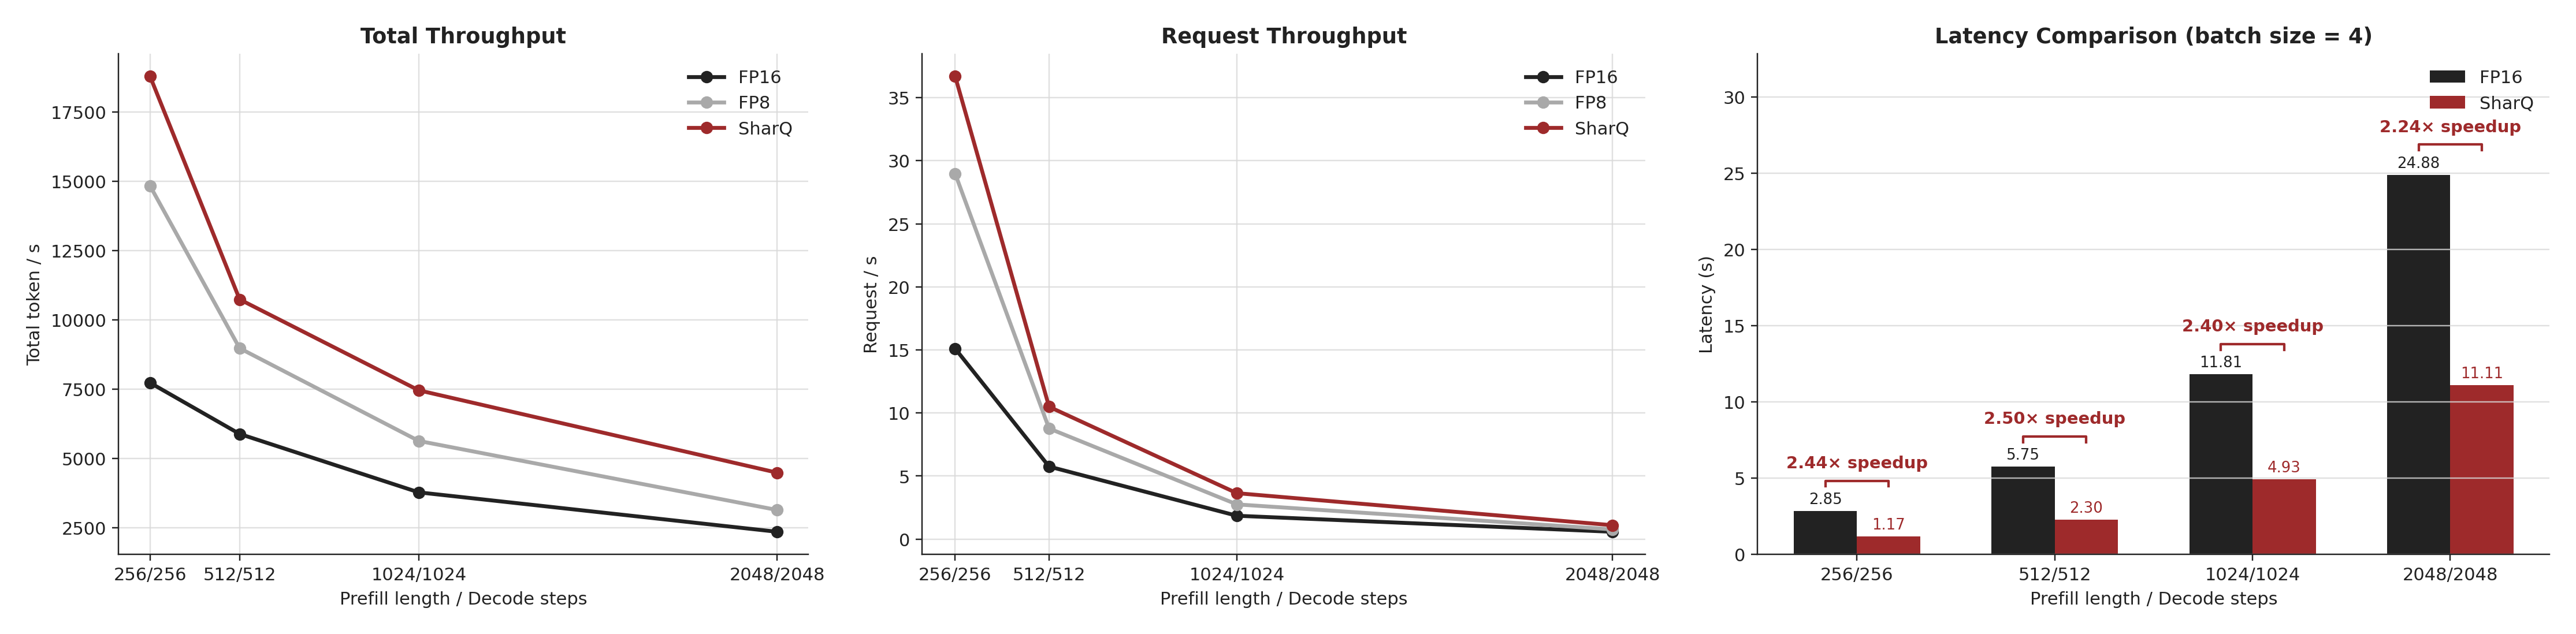
\includegraphics[width=\linewidth]{figures/vllm_efficiency_1x3_red_black.png}
  \caption{vLLM 端到端效率评估。}
  \label{fig:vllm-efficiency}
\end{figure}

\subsection{消融实验}

我们进行两个消融实验来验证 SharQ 的关键设计选择。

\textbf{跨 FP4 格式的泛化性。}
Table~\ref{tab:ablation-format} 在两种不同 FP4 数值格式上评估 SharQ：NVFP4（搭配 4:8 in-pairs 稀疏）和
HiF4（搭配 2:4 稀疏）。在 Qwen3-30B-A3B 上，SharQ 对两种格式都带来稳定改善。对 NVFP4 而言，WikiText2
perplexity 从 9.12 降低到 8.96，LAMBADA accuracy 从 62.91\% 提升到 64.41\%。对 HiF4
也有同样趋势：perplexity 从 9.08 改善到 8.92，LAMBADA 从 63.28\% 提升到 64.08\%。BoolQ
accuracy 在两种格式下也都向 FP16 恢复。这些结果说明 decomposition strategy 与具体格式无关，可以受益于任意
block-scaled FP4 格式与硬件支持的半结构化稀疏组合。

\begin{table}[t]
\caption{SharQ 在不同 FP4 格式上的效果（Qwen3-30B-A3B）。WikiText2 报告 perplexity ($\downarrow$)，其余任务报告 accuracy (\%)。}
\label{tab:ablation-format}
\centering
\small
\begin{tabular}{@{}l|cccc@{}}
\toprule
Method & Wiki2$\downarrow$ & LAMB. & BoolQ & ARC-E \\
\midrule
FP16       & 8.70 & 64.86 & 88.62 & 79.21 \\
\midrule
NVFP4      & 9.12 & 62.91 & 87.77 & \textbf{79.04} \\
SharQ-NVFP4 & \textbf{8.96} & \textbf{64.41} & \textbf{88.41} & 78.58 \\
\midrule
HiF4       & 9.08 & 63.28 & 87.61 & 76.85 \\
SharQ-HiF4 & \textbf{8.92} & \textbf{64.08} & \textbf{88.07} & \textbf{78.07} \\
\bottomrule
\end{tabular}
\end{table}

\begin{table}[t]
\caption{NVFP4 下 sparse--dense 路径组合的消融实验（Llama-3.1-8B）。``Sparse'' 只使用 sparse path，不使用 residual
compensation。``Dense+Dense'' 与 ``Sparse+Sparse'' 使用两条同类型路径。SharQ 将 sparse backbone 与 dense residual 结合。}
\label{tab:ablation-combination}
\centering
\small
\begin{tabular}{@{}l|cccc@{}}
\toprule
Combination & Wiki2$\downarrow$ & MMLU & BoolQ & ARC-E \\
\midrule
Sparse          & 82.95 & 25.78 & 57.03 & 36.74 \\
Dense + Dense   &  \textbf{6.63} & 63.61 & \textbf{81.22} & 76.98 \\
Sparse + Sparse &  6.95 & 61.93 & 79.45 & 77.61 \\
SharQ           &  6.73 & \textbf{63.76} & 80.58 & \textbf{77.74} \\
\bottomrule
\end{tabular}
\end{table}

\textbf{Sparse--dense 路径组合。}
Table~\ref{tab:ablation-combination} 通过在 NVFP4 下改变 sparse 与 dense 计算路径组合，隔离 SharQ
中各路径的贡献。只使用 sparse path 且没有 residual compensation（``Sparse''）会导致灾难性退化：WikiText2
perplexity 上升到 82.95，MMLU 降至 25.78\%，说明直接丢弃所有非 outlier 激活信息会破坏模型质量。``Dense+Dense''
使用两条 dense NVFP4 路径并取得较强精度（WikiText2 6.63，MMLU 63.61），但放弃了半结构化稀疏计算带来的时延收益。``Sparse+Sparse''
使用两条 sparse path，其结果与 NVFP4 baseline 接近（WikiText2 6.95，MMLU 61.93），说明仅增加 sparse
计算而没有 dense compensation signal 并不能恢复稀疏化损失。SharQ 将 sparse backbone 与 dense residual
结合，达到 WikiText2 6.73 和 MMLU 63.76。它在保留 backbone 稀疏执行路径的同时，达到或超过 fully dense two-path
variant 的精度，验证了 asymmetric sparse-plus-dense decomposition 是 SharQ accuracy--efficiency trade-off 的关键。

\section{结论}

\section*{参考文献}

{
\small
}

%%%%%%%%%%%%%%%%%%%%%%%%%%%%%%%%%%%%%%%%%%%%%%%%%%%%%%%%%%%%

\appendix

\section{补充细节}
\section{补充材料}
\subsection{NVFP4 数据格式}
\label{app:nvfp4}

本节介绍实验中作为主要量化目标的 NVFP4 block floating-point 格式。NVFP4 是 NVIDIA Blackwell 架构引入的专有格式，它针对既有
block-scaled FP4 设计的两个关键局限，对 OCP MXFP4 标准进行了改进。

\subsubsection{设计动机}

MXFP4（OCP Microscaling FP4）使用 E2M1 元素、共享的 power-of-two 8-bit exponent（E8M0）以及
32 的 group size，平均存储开销为每个值 4.25 bits。然而，block scale 的 power-of-two 约束不能保证每组峰值都被归一化到
E2M1 的可表示上界，因此会浪费组内动态范围。NVFP4 通过两点设计缓解这一问题：

\begin{enumerate}
\item \textbf{浮点 block scale。} NVFP4 用细粒度 FP8-E4M3 浮点 scale 取代 power-of-two 的 E8M0
scale。这使得 scale 可以更精确地将 group peak 归一化到 E2M1 的上界，从而充分利用组内表达空间。

\item \textbf{更小的 group size。} NVFP4 采用 16 个元素的 group size（相比 MXFP4 的 32 更小），将平均存储开销从
4.25 提高到 4.5 bits/value，但通过更细粒度的缩放显著降低 outlier-driven quantization error。
\end{enumerate}

\subsubsection{格式结构}

一个 NVFP4 block 包含 16 个 4-bit E2M1 元素，它们共享一个 FP8-E4M3 block scale，总存储为
$16 \times 4 + 8 = 72$ bits，即每个值 4.5 bits。E2M1 元素格式为 exponent 分配 2 bits、mantissa
分配 1 bit（normal value 有隐式 leading 1），另有 1 个 sign bit。E2M1 中非零幅值集合为
$\{0.5, 1.0, 1.5, 2.0, 3.0, 4.0, 6.0\}$，最大值为 6，并保留特殊编码表示 $\pm 0$ 和 NaN。

FP8-E4M3 block scale 使用 4 个 exponent bits（bias 为 7）和 3 个 mantissa bits，提供
$[-10, 11]$ binades 的 scale 动态范围（总计 22 binades）。与 E2M1 元素范围结合后，局部组内动态范围为
$\log_2(6/0.5) = 3.58$ binades。

\subsubsection{Per-tensor scaling}

由于 E4M3 block scale 仅提供 22 binades 的全局动态范围，NVFP4 在格式转换前需要额外的软件 per-tensor scaling
(PTS)。PTS 将每个 tensor 的峰值归一化到目标值（activation 通常使用 2688），以保证 E4M3 scale
范围足以覆盖该 tensor 的数值分布。该预处理会在推理中引入一定开销，但对避免 block scale overflow 和 underflow 是必要的。

\subsubsection{稀疏支持}

在 Blackwell 架构上，NVFP4 原生支持 4:8 semi-structured sparsity in pairs。在每 8 个连续元素组成的组中（组织为
4 个 pair），硬件保留 4 个元素（2 个 pair）并裁剪剩余 4 个元素。这种 ``in-pairs'' 约束意味着稀疏选择基于相邻元素 pair
而不是单个值进行，从而简化硬件 metadata encoding，同时仍然可以有效利用 activation sparsity。SharQ 在 NVFP4
实例中正是利用这一 4:8 in-pairs pattern 作为 sparse backbone 约束。

\subsubsection{与其他 FP4 格式的比较}

Table~\ref{tab:nvfp4-comparison} 总结了 NVFP4 与其他 block-scaled FP4 格式的主要差异。

\begin{table}[h]
\caption{Block-scaled FP4 格式设计比较。}
\label{tab:nvfp4-comparison}
\centering
\small
\begin{tabular}{@{}lccc@{}}
\toprule
Feature & MX4 & MXFP4 & NVFP4 \\
\midrule
4-bit Element       & S1P1       & E2M1  & E2M1 \\
Block Scale Format  & E8M0       & E8M0  & E4M3 \\
Group Size          & 16         & 32    & 16 \\
Storage Cost        & 4.0 bits   & 4.25 bits & 4.5 bits \\
Scale Type          & Power-of-2 & Power-of-2 & Floating-point \\
Significand Precision & 2 bits   & 2 bits & 2 bits \\
Local Dynamic Range & 2.81 binades & 3.58 binades & 3.58 binades \\
Global Dynamic Range & N/A       & N/A   & 22 binades \\
Requires PTS        & No         & No    & Yes \\
\bottomrule
\end{tabular}
\end{table}

NVFP4 通过结合 floating-point scale（充分利用 E2M1 可表示范围）和更小 group size（降低 block 内 outlier 影响），相比
MXFP4 获得更好的量化精度。不过，E4M3 有限的全局动态范围要求引入 per-tensor scaling，而更小的 group size
也提高了 metadata 开销。这些 trade-off 使 NVFP4 成为一种面向当前硬件推理精度优化的格式，而 HiF4
（Appendix~\ref{app:hif4}）等格式则探索了更宽动态范围与更低硬件成本的替代设计。

\subsection{HiFloat4 (HiF4) 数据格式}
\label{app:hif4}

本节详细介绍 HiFloat4 (HiF4) block floating-point 格式。它是我们在消融实验（Table~\ref{tab:ablation-format}）中评估的
FP4 数值格式之一。HiF4 被提出作为面向深度学习推理和训练的 high-fidelity 4-bit BFP 格式。为使本文自洽，我们总结其结构、编码方式以及与
NVFP4 的关键差异。

\subsubsection{格式概览}

一个基本 HiF4 单元将 64 个 4-bit in-group 元素与 32 bits 共享缩放 metadata 打包在一起，平均存储开销为每个值
4.5 bits（与 NVFP4 相同）。HiF4 的区别在于其 three-level scaling hierarchy：它同时捕获 group
之间和 group 内部的动态范围变化，相比单层或两层 scale 设计能够提高表示利用率。

%%% PLACEHOLDER: Figure illustrating the HiF4 unit structure %%%
%%% (three-level hierarchy: E6M2 -> E1_8 -> E1_16 -> 64 x S1P2) %%%
% \begin{figure}[t]
%   \centering
%   \includegraphics[width=0.85\linewidth]{figures/hif4_structure.pdf}
%   \caption{HiF4 block floating-point 格式结构。一个 HiF4 单元包含 level-1 E6M2 global base scale、8 个 level-2 one-bit
%   micro-exponents (E1\_8)、16 个 level-3 one-bit micro-exponents (E1\_16)，以及 64 个 4-bit S1P2 scalar elements。}
%   \label{fig:hif4-structure}
% \end{figure}

\subsubsection{三级缩放 metadata}

32-bit scaling metadata 被组织为三个层级：

\textbf{Level-1: Global base scale (E6M2).}
第一层是一个专门设计的 unsigned 8-bit floating-point 格式，称为 E6M2。它为 exponent field 分配 6 bits，bias
为 48；为 mantissa field 分配 2 bits，并使用设为 1 的 hidden integer bit。E6M2 编码 NaN（Not a Number），但不支持
infinity 或 zero；它只使用 normal mode。若记 unbiased exponent 为 $E$，mantissa 为 $M$，则 E6M2 值解释为
\begin{equation}
  X = 2^{E} \times 1.M .
  \label{eq:e6m2}
\end{equation}
该 scale 在 group 之间提供较宽动态范围（unbiased exponent range 为 $[-48, 15]$），并将每组峰值归一化到后续层级结构的可表示上界，从而保证组内动态范围被充分利用。

\textbf{Level-2: 8-way one-bit micro-exponents (E1\_8).}
第二层包含 8 个 one-bit micro-exponents，每个由 8 个连续 in-group 元素共享。每个 E1 bit 编码 1 或 0，表示一个非常细粒度的
power-of-two scaling factor（$2^{E1}$ 即 $2$ 或 $1$）。每个 level-2 E1 进一步连接到两个相邻的 level-3 micro-exponents。

\textbf{Level-3: 16-way one-bit micro-exponents (E1\_16).}
第三层包含 16 个 one-bit micro-exponents，每个由其局部组内 4 个连续 4-bit 元素共享。它们与 level-2 micro-exponents
一起细化组内动态范围，捕获局部 exponent difference，从而有效缓解 outlier 影响并抑制量化误差。

三层 scaling metadata 总计占用 32 bits（$8 + 8 + 16$），分摊到 64 个 in-group 元素上，额外开销为每个值 0.5 bits。

%%% PLACEHOLDER_ENCODING_TABLES %%%

\subsubsection{元素编码：S1P2}

HiF4 使用 sign-magnitude S1P2 表示来编码 64 个 4-bit in-group 元素。在 SXPY 记号中，S 表示 sign bit，P
表示 binary point；P 前面的 X 表示整数部分位数，P 后面的 Y 表示小数部分位数。从概念上看，S1P2 等价于 floating-point 表示中的
E1M2 格式。编码细节见 Table~\ref{tab:hif4-encoding}。

\begin{table}[h]
\caption{HiF4 使用的 E6M2 与 S1P2 编码细节。}
\label{tab:hif4-encoding}
\centering
\small
\begin{tabular}{@{}lcc@{}}
\toprule
Property & Unsigned FP8-E6M2 & Sign-Magnitude S1P2 \\
\midrule
Exponent Bias   & 48              & N/A \\
Unbiased Exp    & $[-48,\;15]$    & N/A \\
Infinity        & N/A             & N/A \\
Zero            & N/A             & $\text{S}0.00_2 = \pm 0.00$ \\
NaN             & $111111\_11_2$  & N/A \\
Max Value       & $111111\_10_2 = 2^{15} \times 1.50$ & $\text{S}1.11_2 = \pm 1.75$ \\
Min Value       & $000000\_00_2 = 2^{-48} \times 1.00$ & $\text{S}0.01_2 = \pm 0.25$ \\
\bottomrule
\end{tabular}
\end{table}

\subsubsection{数值表示}

基于三级层次结构，HiF4 group 中 64 个实数 $\{V_i\}_{i=1}^{64}$ 可以表示如下。若
$\text{E6M2} = \text{NaN}$，则所有 $i \in [1, 64]$ 上都有 $V_i = \text{NaN}$。否则：
\begin{equation}
  V_i
  =
  \text{E6M2}
  \times
  2^{\left(\{\text{E1\_8}\}_{\lfloor i/8 \rfloor}
    + \{\text{E1\_16}\}_{\lfloor i/4 \rfloor}\right)}
  \times
  \{\text{S1P2}\}_i ,
  \label{eq:hif4-value}
\end{equation}
其中 $\{\text{E1\_8}\}_j$（$j \in [1,8]$）和
$\{\text{E1\_16}\}_k$（$k \in [1,16]$）分别表示 level-2 和 level-3 micro-exponents。HiF4
可用的组内动态范围为 $\log_2(7/0.25) = 4.81$ binades，因为 group 内最大正值为
$2^{(1+1)} \times 1.75 = 7$，最小正值为 $2^{(0+0)} \times 0.25 = 0.25$。

\subsubsection{与 NVFP4 的比较}

Table~\ref{tab:hif4-vs-nvfp4} 比较了 HiF4 与 NVFP4 的关键特性。虽然二者平均存储开销相同，HiF4
提供了明显更宽的全局动态范围（69 vs.\ 22 binades）、更高的 significand precision（3 bits vs.\ 2 bits），以及更大的局部动态范围（4.81 vs.\ 3.58 binades）。这些性质使
HiF4 对 outlier-driven quantization error 更鲁棒，并降低了 NVFP4 通常需要的软件 per-tensor scaling (PTS) 需求。

\begin{table}[h]
\caption{HiF4 与 NVFP4 的特性比较。}
\label{tab:hif4-vs-nvfp4}
\centering
\small
\begin{tabular}{@{}lcc@{}}
\toprule
Feature & HiF4 & NVFP4 \\
\midrule
Storage Overhead       & 4.5 bits/value & 4.5 bits/value \\
Group Size             & 64             & 16 \\
Special Values         & NaN and $\pm 0$ & NaN and $\pm 0$ \\
4-bit Element          & S1P2 (E1M2)   & E2M1 \\
Significand Precision  & 3 bits         & 2 bits \\
Global Base Scale      & E6M2           & E4M3 \\
Max Positive Value     & $2^{18} \times 1.3125$ & $2^{11} \times 1.3125$ \\
Min Positive Value     & $2^{-50}$      & $2^{-10}$ \\
Global Dynamic Range   & $[-50,\;18]$: 69 binades & $[-10,\;11]$: 22 binades \\
Local Dynamic Range    & 4.81 binades   & 3.58 binades \\
\bottomrule
\end{tabular}
\end{table}

\subsubsection{从 BF16 转换为 HiF4}

Algorithm~\ref{alg:bf16-to-hif4} 给出了从长度为 64 的 BF16 vector 转换为 HiF4 单元的过程。该算法包含三个阶段：
(1)~三级 tree reduction，用于寻找局部和全局 peak magnitude；(2)~推导三级 hierarchical scaling metadata（E6M2、E1\_8、E1\_16）；
(3)~对 64 个 in-group 元素进行 scaling 并量化为 S1P2 格式。所有 rounding 操作采用 round-half-to-even 或
round-half-away-from-zero。E6M2 reciprocal computation 可以通过由 2-bit mantissa 索引的 4-entry lookup table
加上简单 exponent subtraction 高效实现。

\begin{algorithm}[h]
\caption{从 BF16 转换为 HiF4}
\label{alg:bf16-to-hif4}
\begin{algorithmic}[1]
\REQUIRE 长度为 64 的 BF16 vector $V64$
\ENSURE 一个 HiF4 单元：E6M2, E1\_8, E1\_16, S1P2\_64
\STATE \textbf{// Stage 1: Three-level tree reduction}
\FOR{$i = 1$ to $16$}
  \STATE $V16[i] = \max(|V64[4 \times i - 3 : 4 \times i]|)$
\ENDFOR
\FOR{$i = 1$ to $8$}
  \STATE $V8[i] = \max(V16[2 \times i - 1 : 2 \times i])$
\ENDFOR
\STATE $Vmax = \max(V8)$
\STATE \textbf{// Stage 2: Derive scaling metadata}
\STATE $SF_{BF16} = Vmax \times (1/7)_{BF16}$
  \hfill\COMMENT{高精度缩放因子}
\STATE $\text{E6M2} = \text{BF16\_to\_E6M2}(SF_{BF16})$
  \hfill\COMMENT{Level-1 scale}
\STATE $\text{E6M2\_REC} = \text{E6M2\_REC\_to\_BF16}(\text{E6M2})$
  \hfill\COMMENT{Reciprocal}
\STATE $\text{E1\_8}[i] = (V8[i] \times \text{E6M2\_REC} \geq 4)\ ?\ 1 : 0$
  \hfill\COMMENT{Level-2 scales}
\FOR{$i = 1$ to $16$}
  \STATE $\text{E1\_16}[i] = (V16[i] \times \text{E6M2\_REC} \times 2^{-\text{E1\_8}[\lceil i/2 \rceil]} \geq 2)\ ?\ 1 : 0$
\ENDFOR
\STATE \textbf{// Stage 3: Quantize 64 elements}
\FOR{$i = 1$ to $64$}
  \STATE $V64\_\text{scaled}[i] = V64[i] \times \text{E6M2\_REC} \times 2^{-\text{E1\_8}[\lceil i/8 \rceil]} \times 2^{-\text{E1\_16}[\lceil i/4 \rceil]}$
\ENDFOR
\STATE $\text{S1P2\_64} = \text{BF16\_to\_S1P2}(V64\_\text{scaled})$
  \hfill\COMMENT{量化为 S1P2}
\end{algorithmic}
\end{algorithm}

对于 HiF4 dot product，level-2 和 level-3 micro-exponents 可以在硬件中实现为简单的 left-shift 操作。当集成到原本为
16-bit 和 8-bit 格式优化的 64-length dot-product units 中时，HiF4 只占用约 NVFP4 三分之一的增量面积，并降低约
10\% 功耗，从而为矩阵乘提供更具面积和功耗效率的实现方式。

%%% PLACEHOLDER: Figure comparing HiF4 and NVFP4 dot-product compute flow %%%
% \begin{figure}[t]
%   \centering
%   \includegraphics[width=\linewidth]{figures/hif4_dot_product.pdf}
%   \caption{HiF4 与 NVFP4 的 64-length dot product 计算流程比较。HiF4 在从 64 个 product reduction 到单个 output
%   的过程中使用纯整数运算，仅在最终累加阶段需要一个小型 floating-point multiplier 和一个大型 integer multiplier。}
%   \label{fig:hif4-dot-product}
% \end{figure}

%%%%%%%%%%%%%%%%%%%%%%%%%%%%%%%%%%%%%%%%%%%%%%%%%%%%%%%%%%%%

\newpage
\input{checklist.tex}

\end{document}
